\documentclass[10pt]{beamer}
\usetheme{AnnArbor}
\usepackage[utf8]{inputenc}
\usepackage[spanish]{babel}
\usepackage{amsmath}
\usepackage{xcolor}
\usecolortheme{spruce}
\usepackage{here}
\graphicspath{{./Images/}}
\usepackage{verbatim}
\usepackage{amsfonts}
\usepackage{marvosym}
\usepackage[marvosym]{tikzsymbols}
\usepackage{tikz}
\usepackage{tikzducks}
\usepackage{amssymb}
\usepackage{graphicx}
\usefonttheme{professionalfonts}
\author{Josue Huaroto Villavicencio}
\title{Modelo basado en datos para el potencial de ventilación cruzada en ciudades de alta densidad
en simulación CFD acoplada y aprendizaje automático}
\institute[UNI]{Universidad Nacional de Ingeniería}
\begin{document}
\begin{frame}

\includegraphics[scale=0.05]{./Images/logoUNI.png}
\titlepage
\end{frame}
\begin{frame}{Abstract}
\begin{abstract}
Se desarrolla un modelo CFD acoplado a escala urbana en interiores y exteriores y se define un nuevo índice de ventilación para evaluar el potencial de ventilación natural. Primero, el modelo CFD acoplado está desarrollado para estudiar la ventilación cruzada impulsada por el viento. En segundo lugar, se utilizan seis variables de diseño clave para generar 3840 variaciones de diseño paramétrico para la evaluación de ventilación natural. En tercer lugar, es usado un nuevo índice integrado $CIOI_{v}$ para evaluar la relación de velocidad del viento entre el área interior y el área de referencia exterior. Los modelos $CIOI_{v,F1}$ basados en datos se desarrollan para predecir el potencial de ventilación del edificio interior para un soporte rápido de diseño temprano. En comparación con el modelo de regresión lineal multivariante, el modelo no lineal de aumento de gradiente muestra una precisión de predicción mucho mayor (error de porcentaje absoluto medio = 0.16 con $R^{2}$ = 0.8). En la etapa inicial de diseño, los diseñadores e ingenieros pueden omitir las costosas simulaciones de CFD y usar este modelo de unidad de datos para verificar rápidamente los potenciales de ventilación natural del edificio de diferentes opciones de diseño en un entorno urbano.
\end{abstract}
\end{frame}
\begin{frame}
\frametitle{Introducción}
El incremento de la población mundial y la densidad poblacional ocasionada por las migraciones a las grandes ciudades industrializadas ha generado un incremento significativo en el consumo de energía. Los edificios consumen entre el 30\% y el 40\% de la energía total en el planeta; esto genera un calentamiento global excesivo, y cada vez se requieren mayores cantidades de energía. Reducir el uso de energía urbana se vuelve urgente, por ello la tecnología de ventilación natural se está volviendo cada vez más popular en los edificios, a diferencia de la ventilación mecánica; se utiliza fuerzas naturales para crear flujos de aire dentro y alrededor de los edificios.
\end{frame}
\begin{frame}
\frametitle{Tipos de ventilación natural}
\begin{enumerate}
\item Ventilación impulsada por el viento
\item Ventilación impulsada por flotabilidad
\end{enumerate}
Desde una perspectiva de estrategia de diseño, la ventilación natural incluye ventilación de un solo lado, ventilación cruzada y ventilación de chimenea. Este artículo se centra en la ventilación isotérmica cruzada natural impulsada por el viento. Debido a la naturaleza del viento, es complicado diseñar ventilación natural; sin embargo, la simulación CFD puede proporcionar una forma factible de examinar el rendimiento de la ventilación. Aunque no se encuentra en la construcción de aplicaciones de CFD, otros algoritmos de aprendizaje automático no lineales, como las redes neuronales artificiales (ANN) y las máquinas de soporte vectoriales (SVM) se han utilizado ampliamente en la predicción de energía de edificios y han mostrado predicciones precisas.
\begin{figure}
\centering
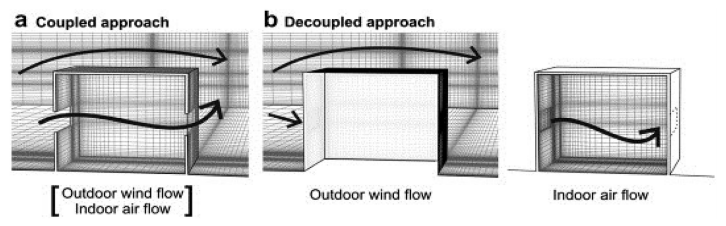
\includegraphics[scale=0.3]{inoutdoot.png}
\end{figure}
\end{frame}
\begin{frame}
\frametitle{Condiciones de frontera}
\begin{eqnarray}
&U(z) =  U_{\mathrm{ref}}\left( \frac{z-z_{0}}{z_{\mathrm{ref}}-z_{0}} \right)^{\alpha} \\[4pt]
&I(z) =  0.1\left( \frac{z}{z_{G}}\right)^{-(\alpha + 0.05)} \\[4pt]
&k(z) \approx  \left[ I_{z}\cdot U_{z} \right]^{2} \\[4pt]
&\varepsilon(z) \approx  P_{k}(z) \approx C_{\mu}^{0.5}k(z) \frac{\mathrm{d}U(z)}{\mathrm{d}z} = \alpha C_{\mu}^{0.5}k(z) \frac{U_{\mathrm{ref}}}{z_{\mathrm{ref}}}\left( \frac{z}{z_{\mathrm{ref}}}\right)^{\alpha - 1}
\end{eqnarray}
Donde $U_{\mathrm{ref}}$ es la velocidad a la altura de referencia, $z_{\mathrm{ref}}$ es la altura de referencia, $\alpha$ es el exponente de potencia basado en la categoría de rugosidad urbana.
\end{frame}
\begin{frame}{Configuración del mallado}
Para reducir la cantidad de elementos en el mallado y reducir el tiempo computacional, se tomo en cuenta medidas simétricas que son inncesarias de recalcular; también se tuvo mallas más finas para las aberturas y bloques de construcción cercanos al objetivo; y una malla más gruesa para el campo lejano.
\begin{figure}
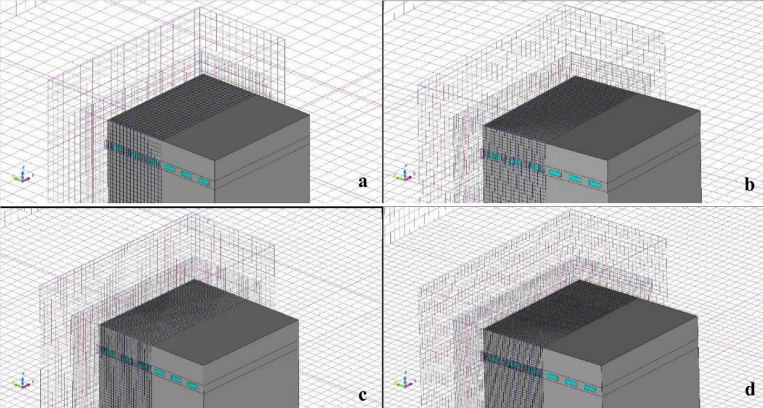
\includegraphics[scale=0.35]{mallado.png}
\end{figure}
\end{frame}
\begin{frame}
\frametitle{Modelos de predicción CIOI}
$$
\mathrm{CIOI} = \frac{\Phi_{in}(x,y,z)}{\Phi_{out,ref}}
$$
CIOI es un parámetro adimensional que se integra los ambientes inteiores y exteriores. Donde $\Phi_{in}(x,y,z)$ es un parámetro interior, como velocidad, presión o concentración de contaminantes en el punto $(x,y,z)$ en el espacio.
\begin{figure}[H]
\centering
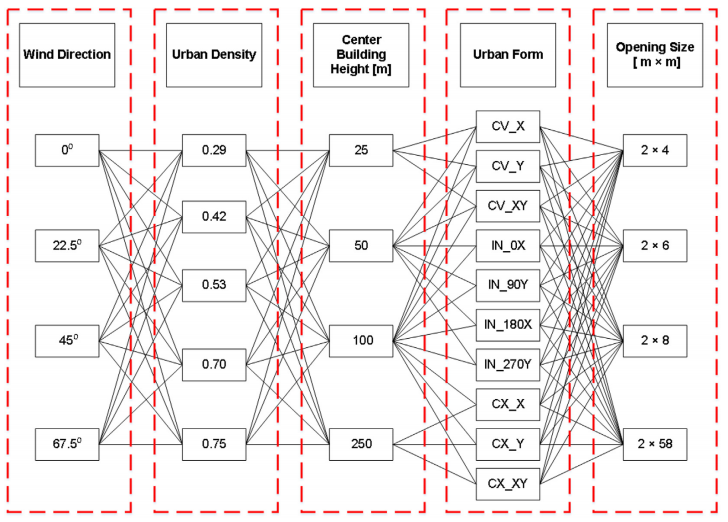
\includegraphics[scale=0.26]{denselayer.png}
\end{figure}
\end{frame}
\begin{frame}[fragile]
\frametitle{Desarrollo del modelo de predicción}
Las simulaciones CFD acopladas pueden proporcionar detalles interiores y exteriores sobre los patrones de viento. Sin embargo, requiere una sólida formación en ingeniería para configurar una simulación y es muy costoso resolver el problema con computadoras tanto en términos de tiempo como de hardware; lo que crea barreras para que los diseñadores las usen. Para hacer rápido un soporte de decisiones disponible en la etapa inicial de diseño, los modelos de aprendizaje automático se generan para predecir $CIOI_{v}$ en base a simulaciones numéricas estocásticas de CFD.\\
El presente modelo fue construido usando datos de la simulación en CFD, 70\% (2688 casos) para entrenamiento y 30\% (1152) para validación.
\end{frame}
\begin{frame}
\frametitle{Métricas del error}
Las siguientes métricas se utilizan para evaluar el rendimiento estadístico de los modelos de regresión.
\begin{itemize}
\item Mean Absolute Error (MAE):
$$
MAE = \frac{1}{N} \sum_{i=1}^{N} \vert \widehat{y}_{i} - y_{i} \vert
$$
\item Root mean square error (RMSE):
$$
RMSE = \sqrt{\frac{1}{N} \sum_{i=1}^{N} (\widehat{y}_{i} - y_{i})^{2}}
$$
\item Normalized root mean square error (NRMSE):
$$
NRMSE = \frac{\sqrt{\frac{1}{N} \sum_{i=1}^{N} (\widehat{y}_{i} - y_{i})^{2}}}{y_{max}-y_{min}}
$$
\end{itemize}
\end{frame}
\begin{frame}
\frametitle{Gradient Boosting}
Debido a la complejidad de las cantidades a predecir, el modelo debe generar regresiones no lineales; sin embargo, se optó por utilizar el Gradient  Boosting como técnica para llegar a predicciones más acertadas. El gradient boosting produce un modelo de predicción en forma de un conjunto de modelos de predicción más débiles. Construye el modelo de manera escalonada como lo hacen otros métodos de refuerzo, y los generaliza permitiendo la optimización de una función arbitraria.
\begin{figure}[H]
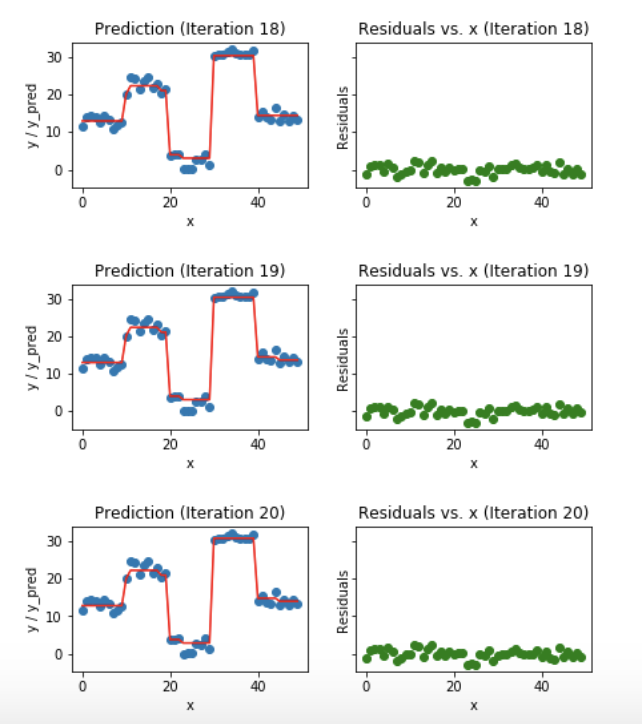
\includegraphics[scale=0.18]{boosting.png}
\end{figure} 
\end{frame}
\end{document}